\documentclass[conference]{IEEEtran}
\IEEEoverridecommandlockouts
% The preceding line is only needed to identify funding in the first footnote. If that is unneeded, please comment it out.
\usepackage{cite}
\usepackage{amsmath,amssymb,amsfonts}
\usepackage{algorithmic}
\usepackage{graphicx}
\usepackage{textcomp}
\usepackage{xcolor}
\usepackage{url}



\def\BibTeX{{\rm B\kern-.05em{\sc i\kern-.025em b}\kern-.08em
    T\kern-.1667em\lower.7ex\hbox{E}\kern-.125emX}}
\begin{document}

% \title{Conditional Synthetic Taxi and Shared Bike Demand Generation for Urban Hubs: Preliminary Work
% }

\title{Multi-Modal Mobility Demand Generation for Urban Hubs: Preliminary Work
}

\author{\IEEEauthorblockN{1\textsuperscript{st} Yuri Frey Hudak}
\IEEEauthorblockA{\textit{Faculty of Mathematics and Computer Sciences} \\
\textit{Eindhoven University of Technology}\\
Eindhoven, The Netherlands\\
y.f.hudak@tue.nl}
\and
\IEEEauthorblockN{1\textsuperscript{st} Anup Vasu Padaki}
\IEEEauthorblockA{\textit{Faculty of Mathematics and Computer Sciences} \\
\textit{Eindhoven University of Technology}\\
Eindhoven, The Netherlands\\
a.v.padaki@tue.nl}
\and
\IEEEauthorblockN{2\textsuperscript{nd} Fabio Paparella}
\IEEEauthorblockA{\textit{Faculty of Mechanical Engineering, Control Systems Technology} \\
\textit{Eindhoven University of Technology}\\
Eindhoven, The Netherlands\\
f.paparella@tue.nl}
\and
\IEEEauthorblockN{3\textsuperscript{rd} Mauro Salazar}
\IEEEauthorblockA{\textit{Faculty of Mechanical Engineering, Control Systems Technology} \\
\textit{Eindhoven University of Technology}\\
Eindhoven, The Netherlands\\
m.r.u.salazer@tue.nl}
}

\maketitle

\begin{abstract}
The design of sustainable multi-modal mobility networks for urban hubs requires further understanding
of the demand for different modes of transport and the relationship between demand and temporal, spatial, and
external factors, such as weather. 
In this paper, we present a preliminary work on the
generation of synthetic demand for taxi and shared bike services in urban hubs. We propose a
conditional synthetic demand generation approach that uses a generative adversarial network to
output synthetic taxi and shared bike demand for the New York City Metripolitan area
conditioned on temporal and weather features. We also compare performance with two traditional variations 
of a multi-output regressor model for the purpose of providing a benchmark for the generative approach.
Our preliminary results show that the proposed 
conditional synthetic demand generation approach is able to generate synthetic taxi and shared bike
demand data conditioned on the basis of weather and temporal features, however further work is
required to improve the quality of the generated data.
\end{abstract}

\begin{IEEEkeywords}
mobility, demand, synthetic data, taxi, bike, shared mobility, urban hubs, NYC
\end{IEEEkeywords}

\section{Introduction}
\subsection{Background:}
As populations migrate away from rural areas and toward urban hubs, mobility 
networks are undergoing large-scale transformations in order to meet this increase 
in demand \cite{secretary_general_sustainable_2018}. These transformations must be 
designed with sustainable objectives in mind, and a number of initiatives have 
investigated sustainable urban mobility systems from a sustainable design perspective
\cite{ghorbanzadeh_sustainable_2019} \cite{canitez_sustainable_2020} \cite{ortuzar_sustainable_2019}. 
Large amounts of funding have been dedicated to advancing sustainable urban mobility 
systems, for example the European Institute of Technology (EIT) recently dedicated 
400 million Euros to investigate the topic \cite{noauthor_eit_nodate}. Numerous initiatives 
are aimed at methods of incentivizing commuters to adopt multi-modal forms of transportation, 
for instance a combination of a subway ride followed by a short e-bike ride. The integration 
of micro-mobility systems within larger urban mobility networks can help cities meet 
increasing demand and reduce traffic congestion from automobiles in a cost-effective 
manner. The introduction of multi-modal micro-mobility systems such as e-scooters and 
e-bikes has also shifted the perception of what form future urban mobility systems might 
take. It has been estimated that micro-mobility providers will comprise a 300- 500 billion 
US dollar market by 2030 \cite{noauthor_future_nodate}.

However, the complex nature of multi-modal mobility in densely-populated urban hubs makes it 
difficult to analyze different trends and preferences of the user toward a mode of transportation. 
The mode of transport that the user chooses is also dependent on various external factors, such as 
weather conditions and time of day, as well as factors internal to the mobility system, such as 
average wait time and total trip time \cite{frank_urban_2008} \cite{beimborn_accessibility_2003}. 
More accurate forecasting models of mobility systems have shown promise as a means of decreasing the 
negative impacts of these internal factors \cite{iglesias_data-driven_2017}. These models can help the 
development of optimal rebalancing and fleet management strategies for fleet vehicles, as well as aid 
further research in the dynamics of urban multi-modal mobility systems. Synthetic datasets which combine
multi-modal mobility systems with external factors such as weather information can also help future 
research in the development of more effective algorithms to address these problems in mobility system 
design.

\subsection{Literature Review:}
In order to provide an overview of the current state of the art in multi-modal mobility demand, we 
review literature in two parts: the development of forecasting models for mobility demand, and the 
generation of synthetic data for mobility demand. 

\subsubsection*{Forecasting:}
There have been several investigations in the areas of short-term taxi demand forecasting using 
Auto-Regressive Integrated Moving Average (ARIMA), a time-series analysis method to predict short-term 
taxi demand \cite{moreira-matias_predicting_2013}. With advances in high-performance computational power, 
Machine Learning and Deep Learning methods \cite{uhrig_sparsity_2017} have been more popular, and have 
yielded promising results \cite{zhang_mlrnn_2022} \cite{hong_spatiotemporal_2021} \cite{liu_improved_2020} 
\cite{rodrigues_beyond_2020} \cite{lai_taxi_2019}. Hybrid approaches where hierarchical clustering algorithms 
have also been demonstrated, for example which showcases a clustering algorithm based on density and distance 
used to construct virtual service 
points and a hybrid network based on convolutional and time-series models used for demand prediction. 
The usage of deep learning attention modules, and specifically transformers \cite{vaswani_attention_2017},
have also paved the way to use architectures like BERT \cite{cao_bert-based_2022}, where demand has been 
predicted by designing the network to learn varying taxi demand patterns between different functional 
regions as 
well as the trends in taxi demand on dynamic daily and weekly time scales. A multi-source 
information-based spatiotemporal  neural network (MSI-STNN) deep learning architecture to predict 
short-term taxi demand has also been  proposed \cite{chen_multi-source_2021}. This model fuses pick-up and 
drop-off time-series data, weather information, 
and location popularity data using three deep-learning models, including a stacked convolutional long 
short-term memory (ConvLSTM) model, a self-attention model, and a convolutional neural network (CNN) 
model. An end-to-end framework has been proposed in \cite{hong_spatiotemporal_2021}, which models the 
spatiotemporal 
correlations with semantic correlations in traffic networks. This approach models five types of spatial 
and semantic correlations into multi-location graphs, which are then fused by a multi-graph convolutional 
network. Temporal correlations between future and past taxi demand values are then captured by an LSTM in 
an encoder-decoder network. Multi-stage learning with LSTMs has also been used to capture pick-up and 
drop-off correlations together with spatiotemporal features to predict pick-up and drop-off
demand \cite{zhang_taxi_2022}. Deep Reinforcement Learning has also been used in taxi demand prediction
to reduce mean waiting times by integrating the derived context through analysis of zone-level taxi 
demands \cite{liu_context-aware_2022}. Travel context has also been modeled from different data sources 
to make demand predictions \cite{liu_contextualized_2019}. Some investigations have modeled point of interest (POI) 
regions to study taxi demand around urban regions with POIs, such as parks or popular destinations
\cite{cao_bert-based_2022}
\cite{askari_taxi_2020} Generative Adversarial Networks (GANs) have also been used recently to solve 
time-series forecasting problems \cite{goodfellow_generative_2014} \cite{jiang_forecasting_2019}. Specifically, 
in \cite{saxena_12d_2022} a stochastic spatio-temporal 
generative model (D-GAN) has been proposed which adopts a GAN-based structure for more accurate 
spatiotemporal prediction in multiple future time steps. This proposed network also supports the 
fusion of external factors through explicit objectives to improve the model learning process. 

\subsubsection*{Synthetic Data Generation:}
Synthetic data generation is a subdomain of data science which has multiple applications including 
data augmentation, data security, style transfer and manipulation, and signal super resolution \cite{surendra_review_2017}. 
As opposed to forecasting network architectures which are designed to predict data for future time steps, 
data generation architectures are intended to produce data which resembles the original distribution of the 
training data. Traditional large dataset generation methods for deep learning applications include the 
variational autoencoder architecture \cite{rezende_stochastic_2014} \cite{kingma_auto-encoding_2014} which 
has been superseded by the generative
adversarial network (GAN) due to its improved performance, however recently the two architectures have been 
combined with promising results \cite{larsen_autoencoding_2016}. A traditional GAN network is comprised of two main components: 
the generator (G) and the discriminator (D) \cite{goodfellow_generative_2014}. The former is an individual network which learns
to generate synthetic data based as closely as possible on the statistical distribution of the real dataset. 
The latter is a separate individual network whose sole objective is to correctly identify output from the 
generator as either real or ‘fake’. Together, the Generator and Discriminator essentially adhere to the 
‘zero-sum game’ model from game theory in which it is theorized that both networks strive for a Nash equilibrium. 
The two are trained iteratively according to the min-max loss function
\begin{equation}
  \min_{G}\max_{D}\mathbb{E}_{x\sim p_{\text{data}}(x)}[\log{D(x)}] + \\ \mathbb{E}_{z\sim p_{\text{z}}(z)}[1 - \log{D(G(z))}]
\end{equation}
where $p_{\text{data}}(x)$ is the distribution of the real data, $p_{\text{z}}(z)$ is the distribution of the
latent space, and $G(z)$ is the output of the generator network. The generator network is trained to minimize
the loss function. The 
discriminator network is, conversely, trained to maximize the loss function. A more formal definition of the binary-crossentropy loss function and its use
in the context of GANs is out of the scope of this paper, however the reader is directed to \cite{goodfellow_generative_2014}
for an in-depth discussion.

In general, there are no constraints on the underlying form that the generator or discriminator networks take, 
however best practices have emerged based on particular domains. The two networks are typically constructed with 
different architectures due to their unique objectives. Training is typically performed in mini-batched samples 
of the training dataset $x$ and the prior noise distribution $z$. The network weights of G and D are updated using
backpropagation, with only one network being trained at once. Architectures vary according to the type of data
being generated, however deep convolutional networks are common and are typically used for image generation.

The development of GANs for spatiotemporal data is a relatively new area of research, but some promising models 
have emerged.  Gao et. al. provide an extensive review on the subject of variations of GAN architecture for the 
spatiotemporal domain \cite{gao_generative_2022}. Saxena and Cao proposed a deep generative adversarial network-based model, 
called D-GAN, which includes a deep spatiotemporal feature learning network and a fusion module for the addition 
of external factors such as weather, points of interest, and weekend vs. weekday \cite{DBLP:journals/corr/abs-1907-08556}.

The development of the conditional GAN (cGAN) builds upon the traditional GAN architecture with the addition 
of a layer for both the generator and discriminator which provides extra information, for example in the form 
of class labels or data from other modalities, which is embedded and combined with the original data \cite{mirza_conditional_2014}. 
In the generator network, the prior input noise $p_{\text{z}}(z)$ is combined with the conditional data in a joint hidden 
representation. Importantly, the conditional GAN allows the targeted generation of synthetic data based on desired 
class characteristics intrinsic to the latent space. In the context of urban mobility planning, this architecture
provides the potential for targeted mobility demand generation based on time, location, weather, and other features.
To the best of the knowledge of the authors, the development of a conditional GAN for the generation of mobility
demand based on time, location, and weather classes has not yet been published.

\subsection{Statement of Contribution:}
Predicting multi-modal mobility demand (e.g. taxi, bike, etc.) is a difficult problem and it is dependent on numerous 
factors. Recent developments in deep learning demonstrate that taxi and bike demand can be predicted more accurately 
through more complex deep learning architectures, together with modules for fusing mobility features, weather information, 
and spatiotemporal features, similar to \cite{zhou_predicting_2018} \cite{prado-rujas_combining_2023}. Synthetic data generation
 for spatiotemporal 
data can be constrained through the addition of conditional class labels, and in this way high-dimensional data distributions
can be learned and generated \cite{mirza_conditional_2014}. Therefore, the main contributions of this paper are as follows:

\begin{itemize}
  \item A preliminary conditional GAN-based deep learning network to fuse spatiotemporal mobility features and weather features 
which can generate synthetic urban taxi and shared bike demand data for variable time periods conditioned on weather class, 
date, and time of day.
  \item A comparison of the proposed conditional GAN architecture with traditional feedforward deep learning regression architectures.
%   \item A querying tool for the conditional generation of synthetic taxi and bike demand data which jointly returns a set of taxi 
% and bike demand estimates.
\end{itemize}

The aforementioned contributions are demonstrated through the application toward two specific mobility networks: the New York 
City (NYC) Yellow Cab system and the New York City CitiBike docked shared bicycle system. All work is available on our public 
GitLab repository \footnote{\url{https://gitlab.tue.nl/20200365/mobilityforecast}}.

\subsection{Organization:}
The remainder of this paper is structured as follows: Section II presents the Methodology, including the architecture of the 
preliminary conditional GAN and feedforward networks and a discussion. Section III presents the Results, including performance 
metrics for the proposed conditional GAN system against the benchmark architectures and findings. Section IV presents the 
Conclusion, which discusses the most important outcomes and their interpretations as well as an outlook on applications of 
the results and proposals for future work.

\section{PRELIMINARY MODELING INVESTIGATION}
The following section presents a description of the design of the proposed conditional data generation algorithm,
 benchmarking algorithm designs, and a discussion of the methods.
\subsection{System Design:}
The system design encompasses the development of the entire conditional data generation algorithm, beginning with preprocessing 
of the datasets, design of the deep learning architecture, and finally methods for training and evaluating the model.
\subsubsection{Data Preparation and Preprocessing}

Data for the NYC Yellow Cab system were obtained from the NYC OpenData website \cite{noauthor_nyc_nodate}, which is a free public
 data repository made available by New York City municipal agencies and partners. The selected dataset contained all trip records
  for the Yellow Cab system in PARQUET format for the entire 2021 year. The data includes features for pick-up and drop-off dates
   and times, locations, trip distances, fare information, and passenger counts. Data for the Citi Bike shared docked bike system
    were obtained from the Citi Bike NYC website \cite{noauthor_citi_nodate}, which is a data repository hosted by the Citi Bike 
    initiative. The data includes features for unique ride identification, start and end time and location, and docking station 
    IDs. The selected dataset contained all trip records for the Citi Bike system in CSV format for the entire 2021 year. Weather
     data was obtained from the Weather Underground website \cite{noauthor_weather_nodate}, which provides publicly available 
     historical weather data on an hourly basis for weather stations within the Weather Underground network. The selected dataset
      contained hourly weather conditions for the KWO35 National Weather Service station over the entire 2021 year. 

Custom data preparation methods were developed in order to read the raw datasets and translate them into consistent formats for 
use in the deep learning architecture. Please see Figure \ref{fig:data} for a graphical overview of the data processing pipeline. 
Erroneous data entries in the form of NaN values or empty values were eliminated from the 
datasets. For each feature, values that fell outside of 3 standard deviations from the mean were considered outliers and were 
removed. Exploratory data analysis was conducted to determine which features held more significance relative to taxi and bike 
demand than others. For the taxi and bike datasets, features for pick-up and drop-off times and locations were selected. For the 
weather dataset, features for time and three categorical weather conditions (clear, rainy, or snowy) 
 were found to be the most significant. 

In order to simplify the data space, taxi trip locational data was converted from unique zone ID (a format used by the NYC Taxi 
and Limousine Commission) to corresponding latitude and longitude, since the Citi Bike dataset was already presented with 
locations in the form of latitude and longitude data. This made correlation and structuring simpler. Both sets of locational 
data were binned into discrete sets of latitude and longitude groups of equal dimension in order to make demand calculation 
simpler. 

Demand for taxi and bike trips was calculated from the feature sets by aggregating trips on a monthly, daily, and hourly basis 
and counting the number of trips for each combination of pick-up and drop-off location for both taxi and bike data. For the cGAN 
network, the data was constructed into a 3D series of spatiotemporal arrays, with X and Y dimensions representing pickup and 
dropoff locations, values representing demand, and the Z dimension representing an array for each individual hour in the set. 
A unique 3D array was constructed for taxi and bike data, and both sets were engineered to match spatial bins and temporal bins 
to allow for synchronous generation of taxi and bike demand. A separate 3D ‘class’ array is constructed which contains the month
 and day as well as the weather conditions for each corresponding hour. A single class array is used for both taxi and bike data,
  since the two datasets were correlated along temporal and spatial dimensions. For the feedforward network, the data is 
  constructed into a 2D array with a column for month, day, hour, unique pickup-dropoff combination, weather conditions, and 
  finally taxi and bike demand. Each row represents an individual hour of data. Both sets of data for the cGAN and feedforward 
  networks contain data for every hour over the course of one full year, in this case 2021.

\begin{figure}[t]
  \centerline{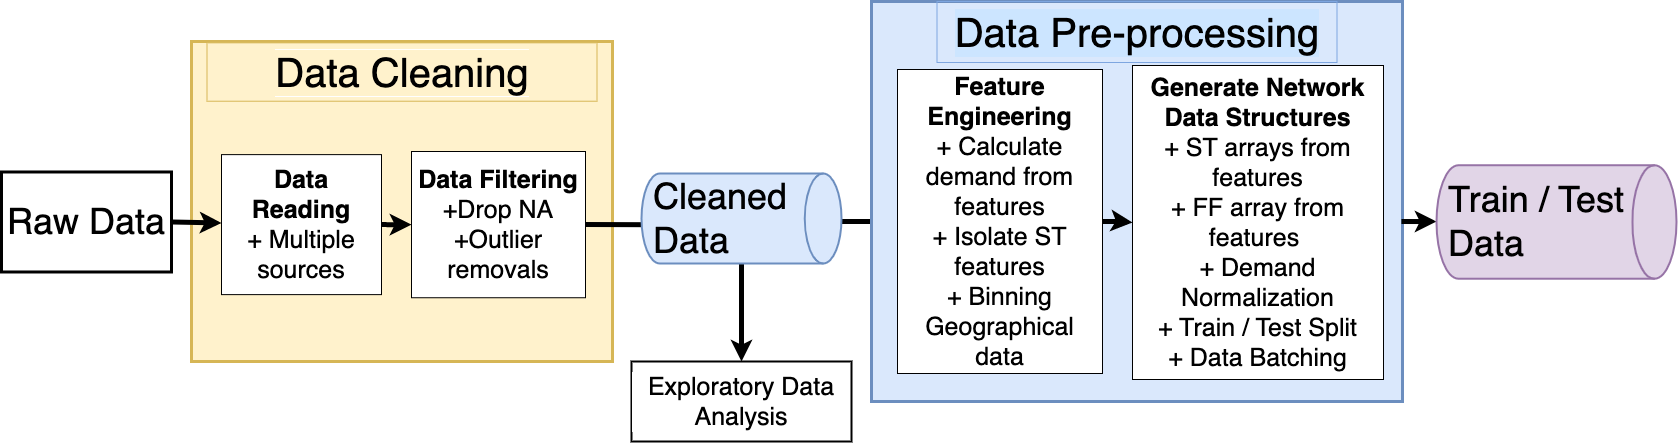
\includegraphics[width=0.5\textwidth]{figs/dataPipeline.png}}
  \caption{Data processing pipeline for cGAN and regression networks.}
  \label{fig:data}
  \end{figure}

\subsubsection{Network Design}
The conditional generative adversarial network (cGAN) consists of two main blocks: the generator and the discriminator, who 
together act as adversaries during the training process. An overview network architecture and training diagram can be seen in Figure
\ref{fig:gan}.
The generator has to goal of generating synthetic data which matches 
the training dataset distribution. The discriminator has the goal of discriminating whether the input data is ‘real’ (from the 
original distribution) or ‘fake’ (produced by the generator). In this preliminary work, the generator network design follows a 
traditional convolutional neural network (CNN) architecture, which was chosen because the data is essentially comprised of low 
resolution images. Throughout this text, the terms image and spatiotemporal array will be used interchangeably. The generator 
also utilizes an embedding layer for the class labels. The generator takes as inputs a latent space dimension and the number of 
classes. The generator outputs a single ‘image’ array (a 2D spatiotemporal array of demand for corresponding pickup and dropoff 
locations) based on the input class labels. The discriminator network design also follows a traditional CNN architecture with an
embedding layer for the class labels. The discriminator takes as input an ‘image’ (a 2D spatiotemporal array) and the number of
classes. The discriminator outputs a single sigmoid prediction in the range of 0 to 1, which predicts whether the input image 
was ‘fake’ or ‘real’ (synthetically generated or from the original distribution).  Both of these networks are then combined in
a simple cGAN network which takes as inputs the generator and discriminator models and tracks training metrics. The conditional
inputs for both the generator and discriminator networks are the class labels for each of the temporal, spatial, and weather 
classes (8 in total). This input is constructed as a 1-dimensional array with a single value for each class label. An embedding 
layer in each network maps the 1D array to a 2D array, and this embedding layer is then fed to a fully connected layer, which
is then reshaped and concatenated with the spatiotemporal array. 

\begin{figure}[t]
  \centerline{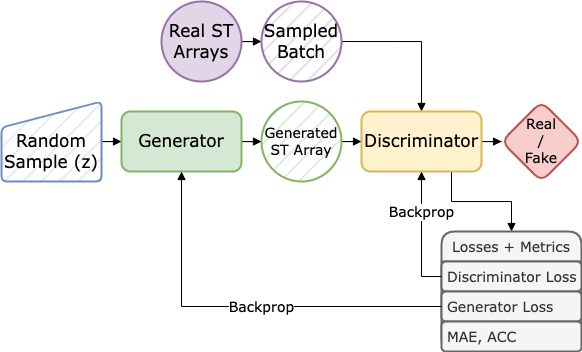
\includegraphics[width=0.5\textwidth]{figs/ganArchitecture.png}}
  \caption{GAN network architecture and training diagram.}
  \label{fig:gan}
  \end{figure}

The feedforward regression network, shown in Figure \ref{fig:ff}, for this preliminary work is formulated as a nonlinear regression network with multiple outputs. It 
follows a traditional multi-layer perceptron (MLP) architecture, with sequential fully-connected layers which reduce the shape of
the network space to two sigmoidal outputs which individually predict a value between zero and one for the normalized taxi and 
bike demand. The network takes as an input a 1D array containing an individual row from the 2D array of training features. A simple 
multi-output regression model was also constructed using the Scikit-learn library \cite{scikit-learn} for comparison.

\begin{figure}[t]
  \centerline{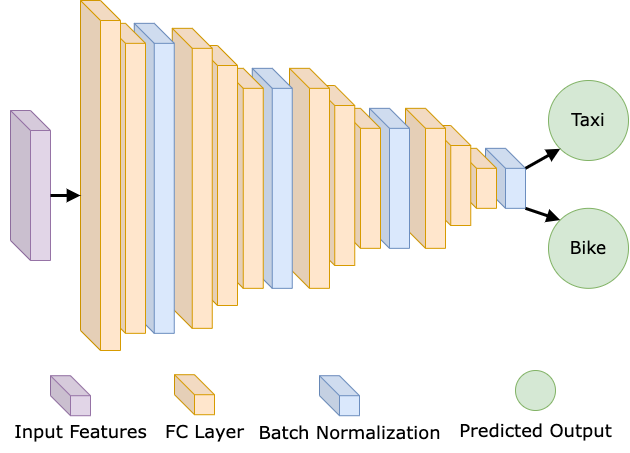
\includegraphics[width=0.5\textwidth]{figs/ffNetwork.png}}
  \caption{Fully-connected feedforward regression network architecture.}
  \label{fig:ff}
  \end{figure}

\subsubsection{Model Training}
The cGAN network was trained using binary crossentropy as the loss function, which essentially gives the network the objective to
 maximize the probability that the spatiotemporal arrays output by the generator are assigned a value of 1, or ‘real’ by the 
 discriminator. The performance metric computed for the cGAN network was mean absolute error (MAE), which applies to the discriminator's class predictions 
 as well as the
 spatiotemporal array distributions output by the generator compared with the training data. The cGAN was trained for 50 epochs,
  and a separate model was trained for taxi and bike demand data. 
The custom feedforward regression network was trained using the mean absolute error for predicted taxi and bike demand values as the 
loss function,
 which gave the network the objective to minimize the difference between predicted and real values for taxi and bike demand. 
 Mean absolute error was also used as the performance metric. The custom feedforward regression network was trained for 50 epochs at a 
 learning 
 rate of 0.1 for both taxi and bike demand data simultaneously. The multi-output regression model from Scikit-learn was also fit to the
 data prepared for the custom regression network and MAE was used as the performance metric.

\subsection{Results and Discussion:}
A summary of performance metric results for the cGAN model and the custom regression model is presented in Table \ref{tab:metrics}. As an additional 
point of comparison, a simple multi-output Regressor model from the Scikit-Learn Python library \cite{scikit-learn} was fit to 
the data used for the custom regression network, and its performance metrics are also included in Table \ref{tab:metrics}. 
Both the custom regression
 network model and the multi-output Regressor model performed reasonably well at predicting values for taxi and bike demand at 
 single points in time. The cGAN taxi and bike models both showed poor performance at the task of generating spatiotemporal 
 arrays of pickup-dropoff demand. A sample of a generated array for an hour of both taxi and bike demand as well as a 
 corresponding sample from the data used for testing the models can be seen in Figure \ref{fig:ganresults}. 
 This poor performance could be due to 
 the large degree of sparsity seen in the training data, for which convolutional-based neural network architectures typically 
 underperform. Future work will investigate methods for addressing this inherent sparsity. 

 \begin{figure}[t]
  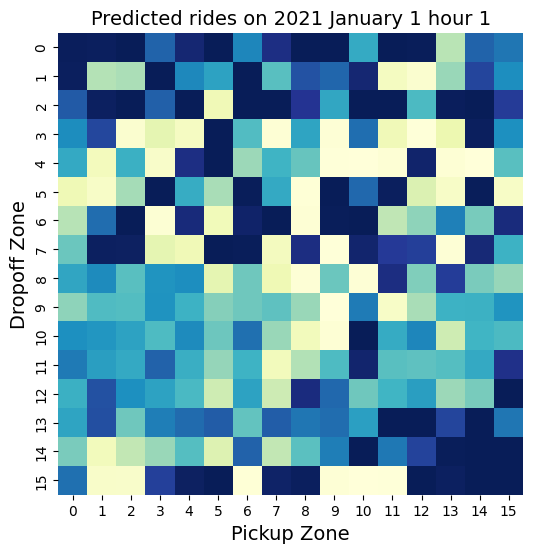
\includegraphics[width=.45\columnwidth]
    {figs/ganpredicted.png}\hfill
  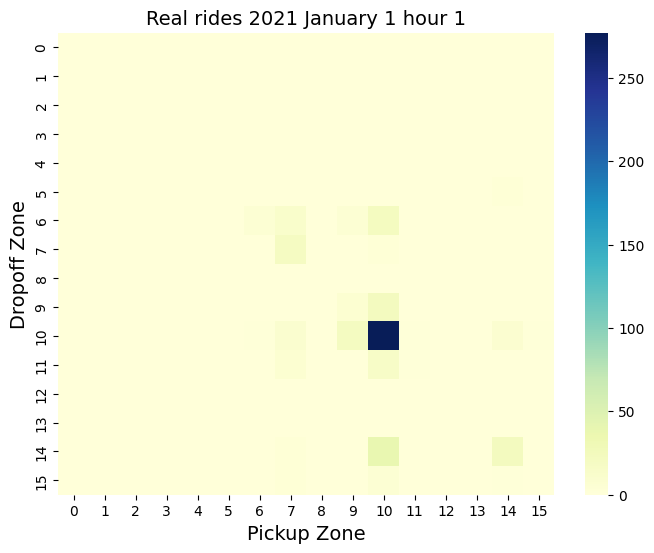
\includegraphics[width=.55\columnwidth]
    {figs/gantest.png}

  \caption{Sample of predicted hour of taxi demand with corresponding sample from the testing data.}
  \label{fig:ganresults}
\end{figure}

 \begin{table}[t]
  \caption{Model Performance Metrics}
  \begin{center}
  \begin{tabular}{|c|c|c|c|c|}
  \hline
  \textbf{Metric} & \multicolumn{2}{|c|}{\textbf{GAN}} & \multicolumn{2}{|c|}{\textbf{Regression}} \\
  \cline{2-5} 
  & \textbf{\textit{Generator}}& \textbf{\textit{Discriminator}} & \textbf{\textit{FF}}
  & \textbf{\textit{Scikit-Learn}}\\
  \hline
  BCE Loss & 26.4 & 0.001 & N/A & N/A \\
  % \cline{1-4} 
  \hline
  MAE & 0.99 & 0.001 & 0.0027 & 0.0042 \\
  \hline
  % \multicolumn{4}{l}{$^{\mathrm{a}}$The Scikit-learn model.}
  \end{tabular}
  \label{tab:metrics}
  \end{center}
  \end{table} 

Further context is warranted to clarify some design choices for the reader. First, the structures given to the training data for
 both the cGAN network and the feedforward regression network were designed according to best practices for both formulation approaches, 
 however there is room for exploration in both cases. Binning of the spatial data into discrete containers of latitude and 
 longitude values is a hyperparameter that will be explored further in future work. In the present preliminary investigation, 
 the spatial data was discretized into 16 bins. Future work will investigate higher resolution bins as well as multi-scale bins
  of variable resolution in urban areas with higher expected demand. In addition, performance comparison of the two different 
  network architectures was limited to the mean absolute error metric for the output demand values for the cGAN and feedforward
   networks. However, due to the high contrast between the two architectures and their respective learning processes, the authors
    will investigate more advances methods of performance comparison in future work. An additional choice made for the training 
    process of the cGAN model was the decision to train the generator network 10 times for every iteration of training the 
    discriminator network. This was done in order to compensate for behavior seen in previous training attempts, where the 
    discriminator clearly dominated the adversarial relationship between the two networks and the generator was unable to 
    produce spatiotemporal arrays capable of fooling the discriminator. This parameter will be investigated further in future 
    work. Lastly, it is important to clarify an assumption made during the data processing and feature engineering stage of 
    this preliminary investigation: the weather features were assumed to be consistent across all spatial dimensions. Due to 
    the small geographical area being considered in the data, the authors chose to simplify the space of the conditional classes
     for weather by assigning conditions from a single weather station located in the Manhattan neighborhood to all locations 
     at each time step.

\section{CONCLUSION}
This paper explored preliminary deep learning architectures for the generation of synthetic data for taxi and bike demand in
 the NYC Metropolitan area across spatial and temporal dimensions together with weather conditions. A preliminary conditional 
 generative adversarial network was designed, trained, and tested. For the purpose of contextual comparison, a traditional 
 multi-layer perceptron feedforward regression network was also designed, trained, and tested on the task of prediction of taxi and bike
  demand values, formulated as a nonlinear regression problem. The performance of the resulting models demonstrated the need 
  for further investigation of the architecture for the conditional GAN network, especially with regard to handling the inherent
   sparsity of the data. However, the cGAN architecture showed promise in its ability to handle complex multidimensional 
   spatiotemporal data and fuse it with weather conditions and date-time labels for the conditional generation of synthetic 
   demand data. Upon further development, this approach has the potential to provide significant aid in the research of 
   multi-modal mobility networks. 
This preliminary investigation will be extended as follows: first, we would like to explore more complex architectures for 
the generator and discriminator blocks of the cGAN network. Architectures that allow for better handling of sparse data will 
be investigated, similar to the investigations presented in \cite{nash_generating_2021} \cite{yan_second_2018} \cite{uhrig_sparsity_2017}.
Second, we will investigate the potential for the cGAN network to be used as a non-deterministic forecasting tool for predicting future 
taxi and bike demand, rather than generating demand for the time period of the training data.
 Third, it is of interest to further 
explore the effect of design choices and hyperparameters including the use of location-dependent weather conditions as well 
as spatial bin resolution, multi-scale binning, and the ratio of generator to discriminator training steps per iteration.

% \begin{thebibliography}{00}
\bibliographystyle{unsrt}
\bibliography{ref}
% \end{thebibliography}

\end{document}